\begin{center}
  {\bf
    \vspace{0.9cm}
    Probability - Exercise Sheet 1 - Probability and Random Experiments\\
    \vspace{0.2cm}
    CHAU Dang Minh
  }
\end{center}

\section{Exercise 2.} \textbf{(Random coloring of a complete graph. Ramsey numbers.)} Let $K_n, n\ge 2$ be the complete graph of $n$ vertices. Let $R(k,l)$ be the smallest integer $n$ such that any two colorings of the edges of $K_n$ with red and blue contains either a red complete subgraph of $k$ vertices or a blue complete subgraph of $l$ vertices. We want to show that $R(k,k)\ge 2^{k/2}$ for all $k\ge 3$.
\begin{enumerate}
  \item Show that $R(2,2)=2, R(3,2)=3, R(3,3)=4$.
  \item Fix $n$ and color randomly the edges of $K_n$ with red and blue. For any $R\subset [n]$ of cardinality $k$, let $K_R$ be the complete subgraph of $K_n$ with vertices in $R$.
        \begin{enumerate}
          \item Give a probabilistic model for the random choice of colors for the edges of $K_n$.
          \item Prove that the probability that there exists $R$ such that $K_R$ is monochromatic is bounded by
                $\binom{n}{k}\frac{2}{2^{\binom{k}{2}}}$.
          \item Prove that if $\binom{n}{k}\frac{2}{2^{\binom{k}{2}}} < 1$, then $R(k,k)> n$.
          \item Prove that for all $k\ge 3$, if $n\le\lfloor 2^{k/2}\rfloor$, then $\binom{n}{k}\frac{2}{2^{\binom{k}{2}}} < 1$.
          \item Complete the proof.
        \end{enumerate}
\end{enumerate}

\textit{Solution.}
\begin{enumerate}
  \item We note that $R(k,l)\ge\max\{k,l\}$. Furthermore, if $m>n$ then $K_m$ contains $K_n$ as a complete subgraph. Hence if $K_n$ has a satisfying coloring, then so does $K_m$. Therefore we only need to find the smallest $n$ such that any coloring of $K_n$ contains either a red complete subgraph of $k$ vertices or a blue complete subgraph of $l$ vertices.
        \begin{itemize}
          \item In any coloring of $K_2$, the only edge is either red (left) or blue (right), hence it contains either a red complete subgraph of 2 vertices or a blue complete subgraph of 2 vertices. Therefore, $R(2,2)=2$.
                \begin{figure}[ht]
                  \centering
                  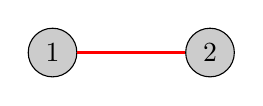
\begin{tikzpicture}
                    \node[circle, draw, fill=black!20] (A) at (0,0) {1};
                    \node[circle, draw, fill=black!20] (B) at (2,0) {2};
                    \draw[red, thick] (A) -- (B);
                  \end{tikzpicture}
                  \hspace{2cm}
                  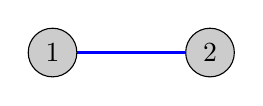
\begin{tikzpicture}
                    \node[circle, draw, fill=black!20] (A) at (0,0) {1};
                    \node[circle, draw, fill=black!20] (B) at (2,0) {2};
                    \draw[blue, thick] (A) -- (B);
                  \end{tikzpicture}
                \end{figure}
          \item The coloring where all three edges are in red satisfies the fact that there is a red $3$-complete subgraph. In other colorings, at least one edge is in blue, which makes a blue $2$-complete subgraph. Therefore, $R(3,2)=3$.
                \begin{figure}[ht]
                  \centering
                  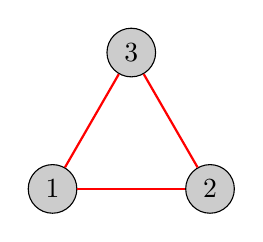
\begin{tikzpicture}
                    \node[circle, draw, fill=black!20] (A) at (0,0) {1};
                    \node[circle, draw, fill=black!20] (B) at (2,0) {2};
                    \node[circle, draw, fill=black!20] (C) at (1,1.732) {3};
                    \draw[red, thick] (A) -- (B);
                    \draw[red, thick] (B) -- (C);
                    \draw[red, thick] (C) -- (A);
                  \end{tikzpicture}
                  \hspace{1cm}
                  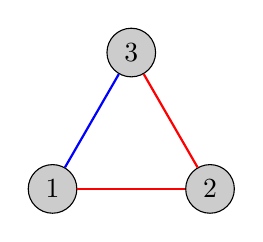
\begin{tikzpicture}
                    \node[circle, draw, fill=black!20] (A) at (0,0) {1};
                    \node[circle, draw, fill=black!20] (B) at (2,0) {2};
                    \node[circle, draw, fill=black!20] (C) at (1,1.732) {3};
                    \draw[red, thick] (A) -- (B);
                    \draw[red, thick] (B) -- (C);
                    \draw[blue, thick] (C) -- (A);
                  \end{tikzpicture}
                \end{figure}
          \item Consider the following coloring of $K_4$. Neither a red $3$-complete subgraph nor a blue $3$-complete subgraph exists. Therefore, $R(3,3)>4$.
                \begin{figure}[ht]
                  \centering
                  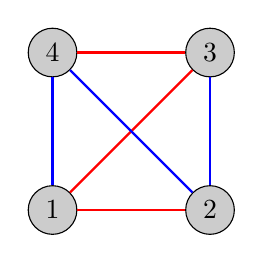
\begin{tikzpicture}
                    \node[circle, draw, fill=black!20] (A) at (0,0) {1};
                    \node[circle, draw, fill=black!20] (B) at (2,0) {2};
                    \node[circle, draw, fill=black!20] (C) at (2,2) {3};
                    \node[circle, draw, fill=black!20] (D) at (0,2) {4};
                    \draw[red, thick] (A) -- (B);
                    \draw[blue, thick] (B) -- (C);
                    \draw[red, thick] (C) -- (D);
                    \draw[blue, thick] (D) -- (A);
                    \draw[red, thick] (A) -- (C);
                    \draw[blue, thick] (B) -- (D);
                  \end{tikzpicture}
                \end{figure}
        \end{itemize}
  \item \,
        \begin{enumerate}
          \item The sample space contains $2^{\binom{n}{2}}$ possible colorings of the edges of $K_n$ i.e.
                $$\Omega = \left\{f \,\middle|\,f: [n]\times [n] \to \{\text{red}, \text{blue}\}\right\}.$$
                We have $|\Omega| = \binom{n}{2}$. The $\sigma$-algebra $\F$ is chosen to be the power set of $\Omega$. The probability measure $\PP$ is uniform on $\Omega$ i.e. for any event $A\in\F$,
                $$\PP(A) = \frac{|A|}{2^{\binom{n}{2}}}.$$
          \item The event that there exists $R$ such that $K_R$ is monochromatic is
                $$E = \bigcup_{\substack{R\subset [n]\\|R|=k}} A_R.$$
                where $A_R$ is the event that $K_R$ is monochromatic. For each subset $R\subset [n]$ of cardinality $k$, we have
                $$|A_R|=2\times 2^{\binom{n}{2}-\binom{k}{2}} = 2^{k+1},$$ since the only two ways to color $K_R$ in a monochromatic way are all red or all blue and for each of these two ways, there are $2^{\binom{n}{2}-\binom{k}{2}}$ ways to color the remaining edges.

                $$\PP(A_R) = \dfrac{2\times 2^{\binom{n}{2}-\binom{k}{2}}}{2^{\binom{n}{2}}} = \dfrac{2}{2^{\binom{k}{2}}}, \forall R\subset [n], |R| = k.$$
                On the other hand, there are $\binom{n}{k}$ ways to choose $R$. By $\sigma$-additivity of $\PP$, we have
                $$\PP(E) = \PP\left(\bigcup_{\substack{R\subset [n]\\|R|=k}} A_R\right) \le \sum_{\substack{R\subset [n]\\|R|=k}} \PP(A_R) = \binom{n}{k}\dfrac{2}{2^{\binom{k}{2}}}.$$
          \item Suppose that $R(k,k)\le n$. Then for any coloring of $K_n$, there exists a red complete subgraph of $k$ vertices or a blue complete subgraph of $k$ vertices. In other words, the event $E$ always happens, i.e. $\PP(E) = 1$. Contrapositively, given that $\PP(E) = \binom{n}{k}\dfrac{2}{2^{\binom{k}{2}}} < 1$, we must have $R(k,k) > n$.
          \item Firstly, notice that for $k \le n < m$, $\binom{n}{k} < \binom{m}{k}$. It is sufficient to show that $\binom{n}{k} < \binom{n+1}{k}$. Equivalently,
                \begin{align*}
                  \dfrac{n!}{k!(n-k)!}        & < \dfrac{(n+1)!}{k!(n+1-k)!} \\
                  \iff (n-k+1)(n-k+2)\ldots n & < (n-k)(n-k+1)\ldots (n+1)   \\
                \end{align*}
                The last inequality is true, since $n-k+i < n-k+i+1$ for all $i=1,2,\ldots,k$. Therefore, it suffices to show that $\binom{\lfloor 2^{k/2}\rfloor}{k}\frac{2}{2^{\binom{k}{2}}} < 1$.

                For $k=3$, we have $\lfloor 2^{3/2}\rfloor = 2\sqrt{2} = 2$. Hence $\binom{\lfloor 2^{3/2}\rfloor}{3}\frac{2}{2^{\binom{3}{2}}} = \binom{2}{3}\frac{2}{2^3} = 0 < 1$.

                For $k=4$, we have $\lfloor 2^{4/2}\rfloor = 4$. Hence $\binom{\lfloor 2^{4/2}\rfloor}{4}\frac{2}{2^{\binom{4}{2}}} = \binom{4}{4}\frac{2}{2^6} = \frac{1}{32} < 1$.

                For $k\ge 5$, we have
                \begin{align*}
                  \binom{\lfloor 2^{k/2}\rfloor}{k}\frac{2}{2^{\binom{k}{2}}}
                   & = \dfrac{\left(\lfloor 2^{k/2}\rfloor-k+1\right)\ldots \lfloor 2^{k/2}\rfloor}{k!}\frac{2}{2^{\binom{k}{2}}}                                                                                                  \\
                   & \le \dfrac{\left(2^{k/2}-k+1\right)\ldots 2^{k/2}}{k!}\frac{2}{2^{\binom{k}{2}}}                                                                                                                              \\
                   & \le \dfrac{2^{k^2/2}}{k!}\frac{2}{2^{k(k-1)/2}} = \dfrac{2^{k/2+1}}{k!} = \dfrac{2^{k/2+1}}{2\ldots k}                                                                                                        \\
                   & \le \dfrac{2^{k/2+1}}{2^{k-1}} = 2^{2-k/2}                                                                                                                                                                    \\
                   & \le                                                                                                                                                                           2^{2-5/2} = \dfrac{1}{\sqrt{2}} \\
                   & < 1.
                  \\
                \end{align*}
          \item Take $n = \lfloor 2^{k/2}\rfloor$, from questions (c) and (d), we have $R(k,k) > \lfloor 2^{k/2}\rfloor$, which means
                $$R(k,k)\ge \lfloor 2^{k/2}\rfloor + 1 > 2^{k/2}.$$
        \end{enumerate}
\end{enumerate}